\documentclass {article}
\usepackage{ragged2e}
\usepackage{graphicx}
\usepackage{subcaption}
\usepackage[utf8]{inputenc}

\graphicspath{ {./images/} }

\title{IT Projekt}
\date{06.05.2019}
\author{Ivaylo Lenkov Ivanov}

\begin{document}

\begin{titlepage}
  \maketitle
  \tableofcontents
  \pagebreak
  \listoffigures
\end{titlepage}

\justify
\section{Einführung}
Für Hauptziel hat dieses Projekt eine virtuelle Umgebung zu bilden und in dieser Umwelt die grundlegende Physik zu simulieren. Die virtuelle Welt ähnelt ein Computerspiel.

\begin{figure}[h]
  \centering
  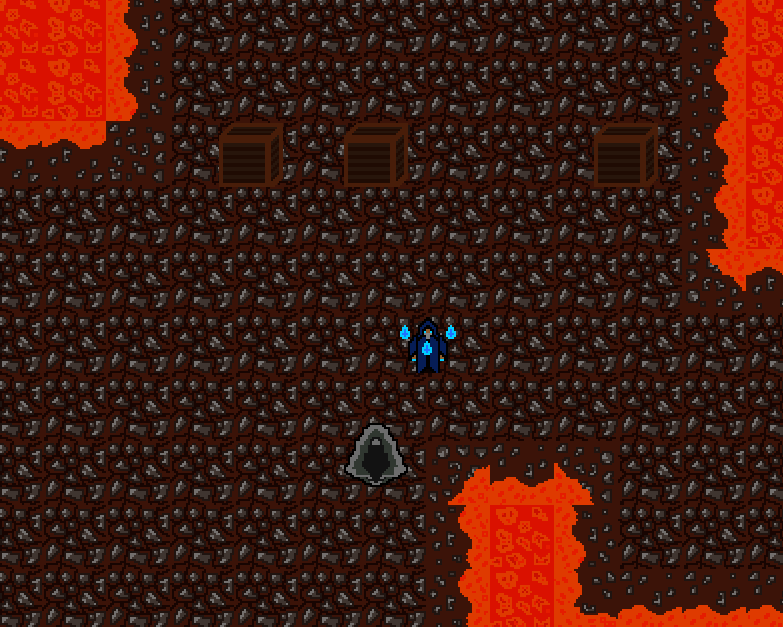
\includegraphics[scale=0.25]{VirtualEnvironment}
  \caption{Die virtuelle Umgebung}
  \label{fig:Umgebung}
\end{figure}

\justify
Der Benutzer steuert eine virtuelle Figur.

\begin{figure}[h]
  \captionsetup{justification=raggedright,singlelinecheck=false}
  
\includegraphics[scale=0.10]{MageCharacter}
  \caption{Avatar}
  \label{fig:Avatar}
\end{figure}

\justify
Der Avatar kann sich in dem Terrain bewegen und Eiszapfen in jeden Richtung feuern. Die Anfangsszene dem Spiel hat vier Spielobjekte --- drei Kasten und ein Stein.

\begin{figure}[h]
  \begin{subfigure}{0.5\textwidth}
    
\includegraphics[width=0.3\linewidth, height=2cm]{Box}
    \caption{Kasten}
    \label{fig:Kasten}
  \end{subfigure}
  \begin{subfigure}{0.5\textwidth}
    
\includegraphics[width=0.3\linewidth, height=2cm]{Stone}
    \caption{Stein}
    \label{fig:Stein}
  \end{subfigure}

  \caption{Spielobjekte}
  \label{fig:Spielobjekte}
\end{figure}

\justify
Mit den Kisten kann der Anwender interagieren. Das heißt, dass der Benutzer sie herumschubsen kann und auch auf sie Eiszapfen zu schießen. Das kann zu der Zerstörung diesen Kästen führen. Der Stein, der auch statisch Spielobjekt genannt wird, funktioniert wie eine Wand. Er ist unbeweglich und auch unverwüstlich.
\end{document}
